\section{Simulation-Based Inference: Approximate Bayesian Computation} \label{sec:abc}
\chedit{
    With our forward model, which includes the \eda~prescription for dust
    attenuation, we can now generate synthetic observations for simulated
    galaxies and make an ``apples-to-apples'' comparison to SDSS. Next, we want
    to use this comparison to infer the posterior probability distribution of
    the \eda~parameters. Typically in astronomy, this inference is done
    assuming a Gaussian likelihood to compare the ``summary statistic''
    (\eg~SMF) of the model to observations and some sampling method (\eg~Markov
    Chain Monte Carlo) to estimate the posterior distribution. The functional form of the
    likelihood, however, depends on the summary statistic and assuming an
    incorrect form of the likelihood can significantly bias the inferred
    posteriors~\citep[\eg][]{hahn2019}. In this work, we use the optical and UV
    color-magnitude relations as our summary statistic. Since the statistic is
    three-dimensional histogram, its likelihood is {\em not} Gaussian but
    rather a Poisson distribution.
}

\chedit{
    Rather than \emph{incorrectly} assuming a Gaussian likelihood or attempting
    to estimate the true Poisson likelihood of the optical and UV
    color-magnitude relations, we use Approximate Bayesian Computation~\citep[hereafter
    ABC;][]{diggle1984, tavare1997, pritchard1999, beaumont2009, delmoral2012}
    for our inference. 
}
ABC is a simulation-based (or ``likelihood-free'') parameter inference
framework that approximates the posterior probability distribution, $p(\theta\given{\rm data})$, without
requiring evaluations of the likelihood.  Instead, ABC only requires a forward
model of the observed data, a prior that can be sampled, and a distance metric
that quantifies the ``closeness'' to the observed data. 
\chedit{
    Since ABC does not require evaluating the likelihood, it does not assume
    any functional form of the likelihood and so we avoid any biases from such
    assumptions. Furthermore, it also allows us to infer the posterior using
    summary statistics with likelihoods that are difficult or intractable to
    directly estimate~\citep{hahn2017a}.
}

In the simplest version of ABC, with a rejection sample
framework~\citep{pritchard1999}, a proposal set of parameter values are drawn
from the prior. The forward model is run with the proposal parameter values.
\chedit{
    The output of the forward model is then compared to the observed data using
    a distance metric that quantifies the ``closeness'' of the forward model
    output to the observed data. 
}
If the distance is within some small threshold, we keep the proposed
parameters; otherwise, we discard them.  Proposals are
drawn until enough pass the threshold to sample the posterior. A
rejection sampling framework requires a large number of evaluations of the
forward model, which
can be computationally costly. Many variations of ABC with more efficient
sampling strategies have now been applied to astronomy and
cosmology~\citep[\eg][]{cameron2012, weyant2013, ishida2015, lin2016, alsing2018}.
Among these methods, we use ABC with Population Monte Carlo (PMC) 
importance sampling~\citep{hahn2017a, hahn2017b, hahn2019a}.

ABC-PMC begins with an arbitrarily large threshold $\epsilon_1$ and $N$ proposals 
$\bar{\theta}_1$ sampled from the prior distribution. Each proposal is
assigned a weight $w^i_1 = 1/N$. Then for subsequent iterations ($n > 1$), the 
threshold, $\epsilon_n$, is set to the median distance of the previous iteration's
proposals. New proposals are drawn from the previous iteration's proposals perturbed 
by a kernel and kept if their distance is blelow $\epsilon_n$. This is repeated
until we assemble a new set of $N$ proposals $\bar{\theta}_n$. The entire
process is repeated for the next iteration until convergence is confirmed. 
We use the Python implementation of
\cite{akeret2015}\footnote{https://abcpmc.readthedocs.io/en/latest/index.html}.
For further details on the ABC-PMC implementation, we refer readers to \cite{hahn2017b}
and \cite{hahn2019a}.

\begin{figure}
\begin{center}
    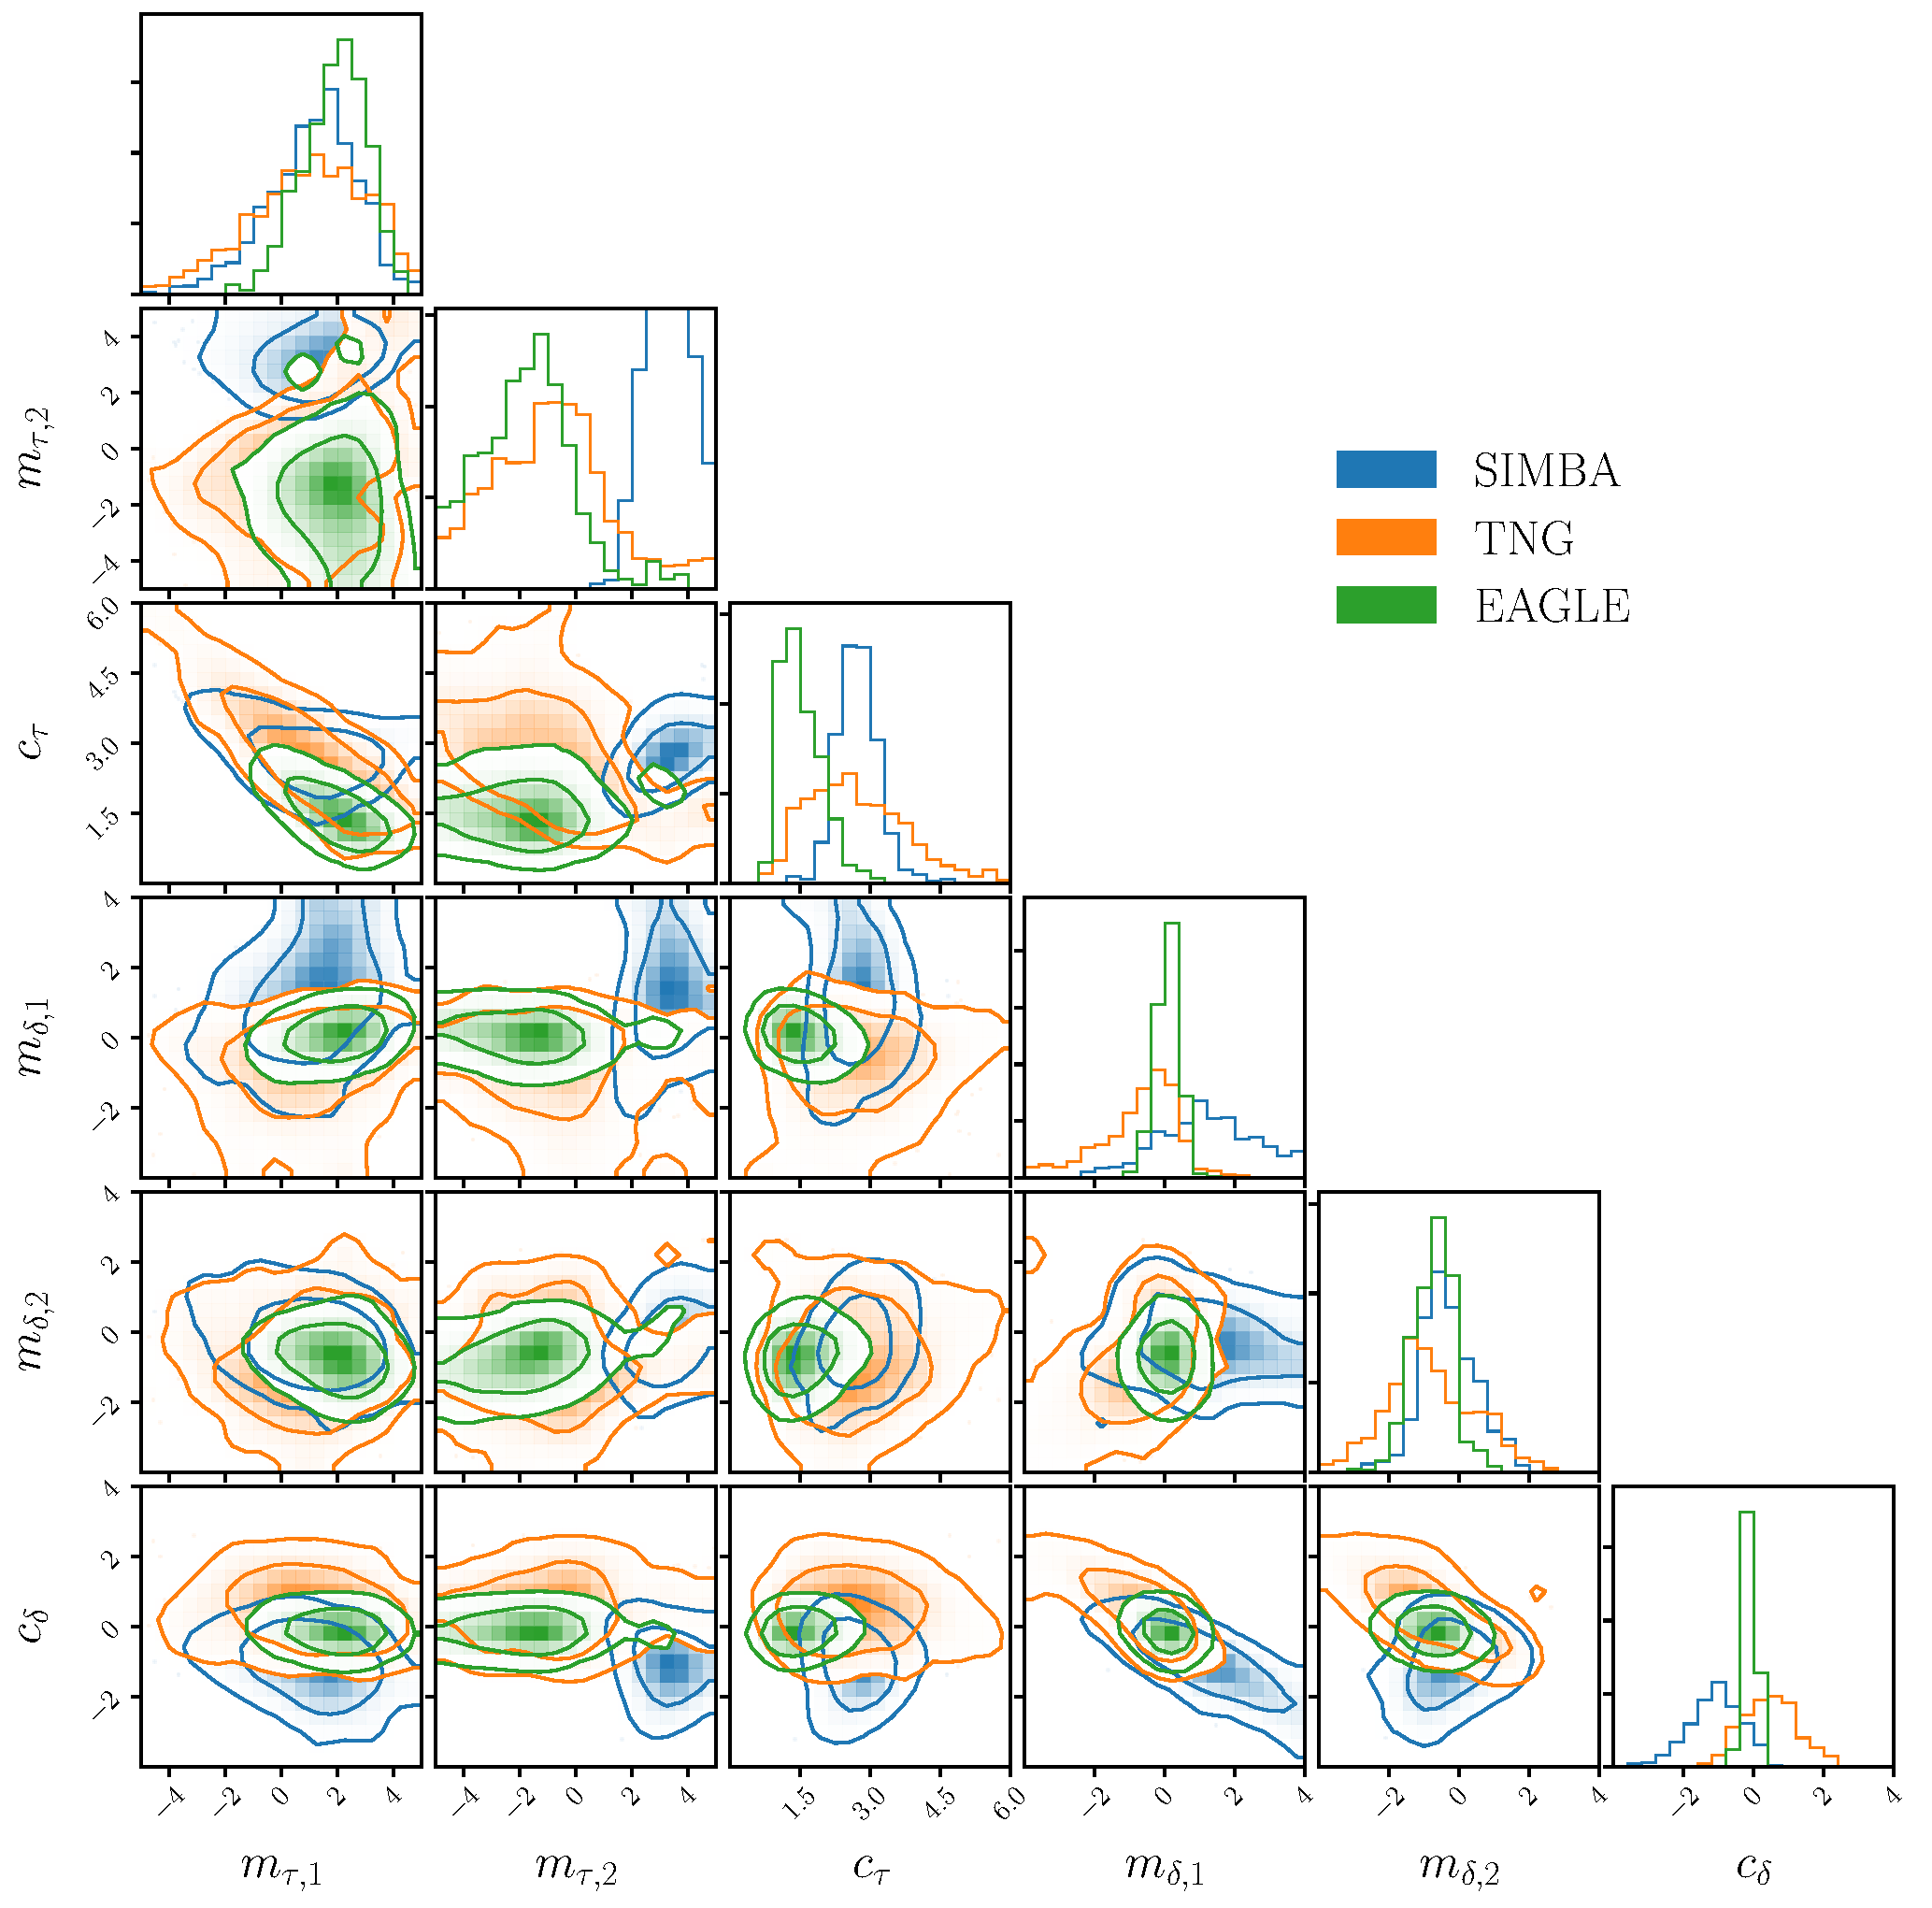
\includegraphics[width=\textwidth]{figs/abc.pdf}
    \caption{\label{fig:abc}
    Posterior distributions of the \eda~parameters for the SIMBA (orange), TNG
    (blue), and EAGLE (green) hydrodynamical simulations. The contours mark the $68$
    and $95$ percentiles of the distributions. The posteriors are derived using the
    simulation-based inference method: Approximate Bayesian Computation with
    Population Monte Carlo (Section~\ref{sec:abc}). We focus on the
    \eda~posteriors for TNG and EAGLE since the \eda~struggles to reproduce
    SDSS observations with SIMBA, which predicts an overabundance of starburst
    galaxies. Based on the posteriors, we find that \emph{galaxies with higher
    $M_*$ have overall higher dust attenuation and galaxies with higher $\ssfr$
    have steeper attenuation curves.}
    }
\end{center}
\end{figure}

\chedit{
    In this work, we use ABC-PMC with uninformative uniform priors on each of
    the \eda~parameters and choose ranges that encompass constraints in the
    literature.
}
The prior ranges of $\mtaum, \mtaus, c_\tau$ are chosen to
conservatively include the $A_V$ range and $M_*$ and $\sfr$ dependence of
\cite{narayanan2018} and \cite{salim2020}. Meanwhile, the prior ranges of 
$\mdeltam, \mdeltas, c_\delta$ are chosen to conservatively include the $\delta$
range and $M_*$ and $\sfr$ dependence of \cite{leja2017} and \cite{salim2018}. 
We list the range of the priors in Table~\ref{tab:free_param}. 
\chedit{
    For our forward model, we use the model described in
    Section~\ref{sec:fm}: we construct SEDs for every simulated galaxies from
    the hydrodynamic simulations, apply dust attenuation with our
    \eda, calculate the observables ($M_r$, $\gr$, and $\fnuv$),
    add uncertainties to them, and apply a $M_r < -20$ completeness 
    limit. 
    We use the optical and UV color-magnitude relation, $(\gr)- M_r$ and
    $(\fnuv)-M_r$ as our summary statistic to fully exploit the $(M_r, \gr,
    \fnuv)$ observational-space. We measure the color-magnitude relations by
    calculating the number density in bins of $(\gr, \fnuv, M_r)$ with widths
    $(0.0625, 0.25, 0.5)$ mags. For our distance metric, $\rho$, we use the L2
    norm between the summary statistics of 
    the SDSS observation, $X^{\rm SDSS}$ and of our forward model, $X^{\rm
    FM}(\theta_{\rm \eda})$: 
}
\begin{equation} \label{eq:distance}
    \rho(\theta_{\rm \eda}) = \left[X^{\rm SDSS} - X^{\rm FM}(\theta_{\rm
    \eda}) \right]^2.
\end{equation}
In Figure~\ref{fig:abc}, we present the posterior distributions of the \eda~parameters
derived using ABC-PMC for the SIMBA (orange), TNG (blue), and EAGLE (green) hydrodynamical 
simulations. The contours mark the $68$ and $95$ percentiles of the distributions. 
